\subsection{Ballistic Rocket}\label{sec:example-ballistic-rocket}

This example simulates a two-stage ballistic rocket trajectory that maximizes impact
velocity.  The rocket is rail launched, but the best launch-rail elevation is unknown.
The second stage is fired downward after apogee to increase impact velocity, but the
firing time and vehicle attitude at ignition are also unknown.  Payload separation
must occur above the atmosphere, second-stage burnout must occur before payload
separation, and final range must be 60 nautical miles.  Optimization is used to solve
for the unknown values while satisfying these constraints.  The trajectory of the
first-stage booster after separation is also calculated to illustrate multiple-vehicle
analysis.

The first stage has a Castor main motor and two smaller Recruit motors.  The Recruits
burn out and are jettisoned at 3 seconds.  The Castor continues to burn for about
40 seconds.  Because the first stage is aerodynamically spin stabilized by fins, it is
not separated until the vehicle is above the atmosphere, assumed here to be
300,000 ft.  After separation, an attitude-control system points the second stage to
its firing attitude.  The vehicle coasts past apogee, the second stage fires downward,
and a short coast after burnout ensures that thrust has ended before the payload is
released to reenter the atmosphere.

The required table files are not printed because they are too large.  Tables are needed
for the thrust and mass flow of the first- and second-stage motors.  Separate drag
tables are needed for the different vehicle configurations, and different tables are
used while a motor is firing and while the vehicle is coasting.

\taossubhead{Problem File}

The problem file is

\lstinputlisting[style=taosmanual,basicstyle=\ttfamily\scriptsize]{examples/chapter04/ballistic-rocket-source.prb.txt}

The file begins, like other problems, with a problem name, title, atmosphere model,
and earth model.  Trajectory 1 simulates the complete vehicle flight; trajectory 2
simulates the first-stage booster as it falls to earth after separation.

\taossubhead{Rail Launch}

The initial conditions for trajectory 1 place the vehicle at zero longitude and
latitude, heading east, because a specific launch site has not yet been selected.  The
launch elevation is an optimization parameter because the best value is unknown.

The trajectory is divided into ten segments.  The first two simulate the rail launch.
Two segments are used because the coefficient of friction changes instantaneously
when the vehicle begins moving.  Segment 1 covers the time from ignition until
thrust overcomes static friction and gravity.  At its end the vehicle has just begun to
move.  Segment 2 continues to the end of the rail, defined by the path-length final
condition.

\taossubhead{First-Stage Burn}

Segment 3 propagates from the end of the launch rail until the Recruit motors are
jettisoned.  During the first three segments, both the Castor and the Recruits are
burning.  Their thrust and mass-flow data are in separate tables, so two
\problemblock{*prop} blocks are evaluated and summed to obtain the total thrust.

The Recruits are jettisoned at the start of segment 4.  A
\problemblock{*increment} block accounts for the weight change, the drag table is
changed because the configuration has changed, and the Recruit propulsion blocks
are removed.  Segment 5 coasts to 300,000 ft using a power-off drag table.  An
additional final condition, \texttt{gamgd<0}, terminates the segment if the vehicle
cannot reach 300,000 ft, preventing a possible infinite segment.

The first stage is separated at the beginning of segment 6.  That segment provides a
30-second margin for the attitude-control system to orient the vehicle before
second-stage ignition.

\taossubhead{Second-Stage Burn}

In segment 7 the vehicle is assumed to have reached the correct firing attitude.
Although segment 6 provides time for the maneuver, the example treats the attitude
change as instantaneous between the two segments.  In segment 6 the body is aligned
with the velocity vector; in segment 7 it is oriented at an unknown geodetic pitch.
That pitch and the amount of coast time before ignition are optimization parameters.

The second stage fires in segment 8.  Its inertial attitude is held constant using the
\statevar{pitchi}, \statevar{yawi}, and \statevar{rolli} guidance rules.  Asterisks
carry the values from the end of the preceding segment into the burn segment.
Segment 9 accounts for the time between burnout and payload separation.  Separation
is delayed until altitude is below 300,000 ft on descent, and segment 10 then
propagates the payload ballistically to impact.

\taossubhead{Trajectory Number 2}

The second trajectory obtains its initial state from trajectory 1 at the beginning of
segment 6, when first-stage separation occurs.  It contains only one segment because
it simply follows the empty first-stage motor from separation to impact; no other
significant events occur.

\taossubhead{Optimization}

The \problemblock{*optimize} block sets maximum impact velocity as the objective.
The altitude at the end of second-stage burnout, segment 8, is constrained to
450,000 ft, and final range at the end of segment 10 is constrained to 60 nautical
miles.  The objective is referenced by 10,000, and a maximum of 30 iterations is
specified.  With only three parameters, the problem should not require many
iterations.

Initial estimates and upper and lower limits are supplied for all three parameters.
Preliminary calculations with optimization disabled by \texttt{maxitr=0} were used
to obtain those estimates.  They need not be highly accurate; they need only produce
a reasonable starting trajectory.

\taossubhead{Results}

The source problem converged in 12 iterations and required 5 minutes 30 seconds on
a Silicon Graphics workstation.  The manual prints the first portion of trajectory 1,
reproduced below as semantic text:

\begin{center}
\begin{minipage}{0.98\linewidth}
\lstinputlisting[style=taosmanual,basicstyle=\ttfamily\tiny]{examples/chapter04/ballistic-rocket-printout.txt}
\end{minipage}
\end{center}

Figures \ref{fig:example-rocket-altitude-range} and
\ref{fig:example-rocket-velocity-time} show the two trajectories written to the EGS
database.  The solid curve is the main vehicle and the dotted curve is the separated
first-stage booster.

\begin{figure}[htbp]
  \centering
  \resizebox{0.84\linewidth}{!}{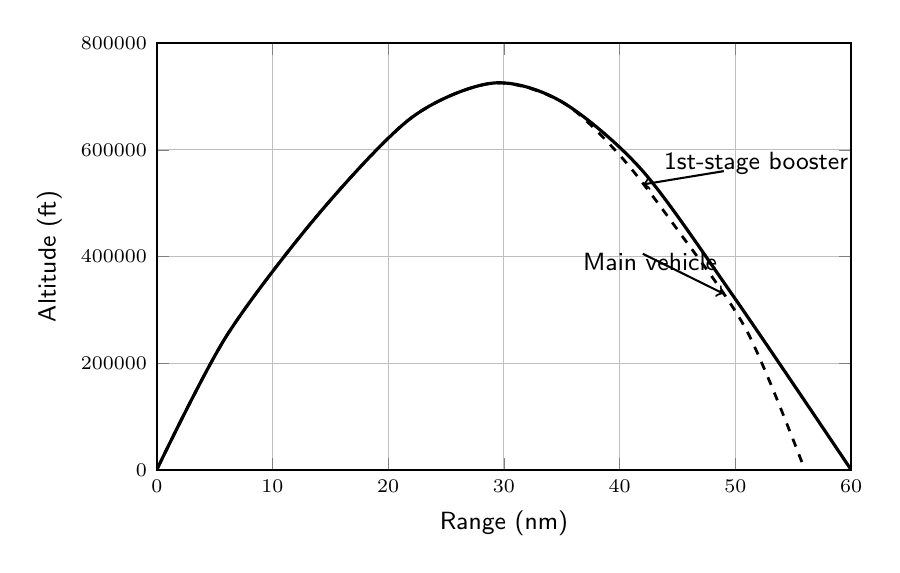
\begin{tikzpicture}
\begin{axis}[
  width=10.4cm,height=7.0cm,
  xmin=0,xmax=60,ymin=0,ymax=800000,
  xtick={0,10,20,30,40,50,60},
  ytick={0,200000,400000,600000,800000},
  grid=major,
  axis line style={line width=0.8pt},
  tick label style={font=\scriptsize},
  label style={font=\sffamily\small},
  xlabel={Range (nm)},ylabel={Altitude (ft)},
  scaled y ticks=false,
  yticklabel style={/pgf/number format/fixed,/pgf/number format/1000 sep={}},
]
  \addplot[line width=1.15pt,smooth] coordinates {(0,0) (6,250000) (14,480000) (22,660000) (29,725000) (35,690000) (42,560000) (50,320000) (60,0)};
  \addplot[line width=1.0pt,dashed,smooth] coordinates {(0,0) (6,250000) (14,480000) (22,660000) (29,725000) (35,690000) (40,590000) (45,450000) (51,260000) (56,0)};
  \node[font=\sffamily\small,anchor=west] at (axis cs:43,575000) {1st-stage booster};
  \draw[->,line width=0.75pt] (axis cs:49,560000)--(axis cs:42,535000);
  \node[font=\sffamily\small,anchor=west] at (axis cs:36,390000) {Main vehicle};
  \draw[->,line width=0.75pt] (axis cs:42,405000)--(axis cs:49,330000);
\end{axis}
\end{tikzpicture}
}
  \caption{Altitude versus range for the example ballistic rocket.}
  \label{fig:example-rocket-altitude-range}
\end{figure}

\begin{figure}[htbp]
  \centering
  \resizebox{0.84\linewidth}{!}{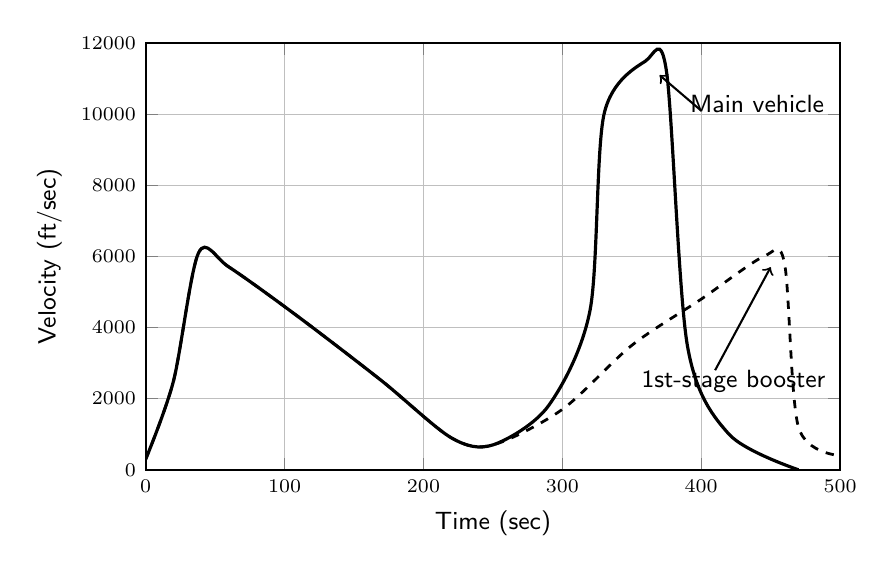
\begin{tikzpicture}
\begin{axis}[
  width=10.4cm,height=7.0cm,
  xmin=0,xmax=500,ymin=0,ymax=12000,
  xtick={0,100,200,300,400,500},
  ytick={0,2000,4000,6000,8000,10000,12000},
  grid=major,
  axis line style={line width=0.8pt},
  tick label style={font=\scriptsize},
  label style={font=\sffamily\small},
  xlabel={Time (sec)},ylabel={Velocity (ft/sec)},
  scaled y ticks=false,
  yticklabel style={/pgf/number format/fixed,/pgf/number format/1000 sep={}},
]
  \addplot[line width=1.15pt,smooth] coordinates {(0,300) (20,2500) (38,6100) (60,5700) (110,4300) (170,2500) (220,900) (250,700) (290,1800) (320,4500) (330,10000) (360,11500) (375,11200) (390,3500) (420,1000) (470,0)};
  \addplot[line width=1.0pt,dashed,smooth] coordinates {(0,300) (20,2500) (38,6100) (60,5700) (110,4300) (170,2500) (220,900) (250,700) (300,1700) (350,3500) (400,4800) (445,6000) (460,5800) (470,1200) (500,400)};
  \node[font=\sffamily\small,anchor=west] at (axis cs:385,10300) {Main vehicle};
  \draw[->,line width=0.75pt] (axis cs:400,10100)--(axis cs:370,11100);
  \node[font=\sffamily\small,anchor=west] at (axis cs:350,2500) {1st-stage booster};
  \draw[->,line width=0.75pt] (axis cs:410,2800)--(axis cs:450,5700);
\end{axis}
\end{tikzpicture}
}
  \caption{Velocity versus time for the example ballistic rocket.}
  \label{fig:example-rocket-velocity-time}
\end{figure}
